% @Author: YangZhou
% @Date:   2017-06-20 20:27:38
% @Last Modified by:   YangZhou
% @Last Modified time: 2017-06-30 19:24:39
\documentclass[%
 reprint,
 amsmath,amssymb,
 aps,
prb,
]{revtex4-1}
\preprint{APS/123-QED}
\usepackage{graphicx}% Include figure files
\usepackage{bm}% bold math
\newcommand{\angstrom}{\mbox{\normalfont\AA}}
\begin{document}
\title{Crystal-amorphous interface induced by graphene nano-knot}
\author{Yang Zhou${}^{1,2}$}
\author{Zhi-Xin Guo${}^{3}$}
\author{Shi-you Chen}
\author{Hongjun Xiang}
\author{Xin-Gao Gong${}^{1,2}$}
\email{xggong@fudan.edu.cn}
\affiliation{%
  ${}^1$Key Laboratory for Computational Physical Science (Ministry of Education), State Key Laboratory of Surface Physics and Department of Physics, Fudan University, Shanghai 200433, China\\
  ${}^2$Collaborative Innovation Center of Advanced Microstructures, Nanjing 210093, Jiangsu, China\\
  ${}^3$Department of Physics, Xiangtan University, Xiangtan 411105, China
}%
\begin{abstract}
  Mechanical and thermal transport properties of graphene nanoribbon knots, are systematically investigated using nonequilibrium molecular dynamics. It is found that the thermal conductivity of the ribbon decreases largely due to the presence of the knots as a defect, but with the increasing of strain, the Kapitza resistance decreases, which is due to a tighter contacting of the ribbon with itself or the other. Local phonon analysis is applied to the contacting regime to reveal the influence of the contacts on the transport. This work would be helpful for a deeper understanding of thermal conducting at nanoscale and give a guidance to the field of phonon management material design.
  \begin{description}
    \item[Keywords]
          Thermal conductivity,graphene, knot , molecular dynamics ,amorphous
  \end{description}
\end{abstract}

\maketitle

\section{INTRODUCTION}

From ancient times knots have been an interesting topic. At begining people invented knots from securing a rope, to build a wood house or prevent animals from eacaping , while others use them to count or art\cite{Adams1995}.
\cite{DietrichBuchecker1989}
Many experiments have been done to determine the relative strengths of different knots, and these show that the break in a knotted rope almost invariably occurs at the point just outside the 'entrance' to the knot.Little is known about the structure and properties of
knots at the atomic level. For example, the minimum number of carbon atoms that can be sustained as a tre- foil in a polyethylene strand is not well established.The influence of knots on
the properties of polymers has become of great interest, in part because of their effect on mechanical Knots are fascinating non-trivial topological entities.They are not only present in art and history but in many scientific fields as well, from mathematics to biology.
properties.Knots (1) form spontaneously in flexible  polymer chains (2) and are found in circular DNA (3)and \~1\%ofproteinsinthe ProteinData Bank (PDB) (4)
Whereas they can appear spontaneously [4] and are sometimes regarded as a nuisance (e.g., in hair and during knitting), knots as fasteners of filamentary structures have applications in biophysics [5], surgery [6,7], fishing [8], sailing [9], and climbing [10]. Frictional
In 1994, Liang and Mislow presented fascinating discussions on knots and
links in relation to chirality [9–10].This breakthrough work should help bridge the gap between the communities of mathematical topologists and molecular chemists.Besides naturally occurring DNA catenanes and knots,a fascinating family of
related molecules has been synthesized and described by Seeman and coworkers [20]
Knots have been created at the molecular level,11,12 a recent synthetic improvement allowing their preparation at a truly
preparative scale13 (0.3 g per batch). The development of this new procedure led us to attempt the resolution of the molecular trefoil knot K,
A number of experimental techniques have been developed
to study knots, particularly in DNA. Knots have been induced with high electric fields11, optical tweezers12,13, topoisomerase enzymes14–16, DNA recombinases17 and through the cyclization of linear DNA molecules18,19. Electron
Graphene and graphene nanoribbon (GNR) are the key role of condensed matter physics because of its excellent mechanical, electrical, and thermal properties. For example, the strength of a graphene ribbon is $10F/m^2$ which is able to hangup a 10t car even if its only 1us width. And the Thermal conductivity is $5000W/mK$ at room temperature, making it the most conducting material in this world.
Despite this interest, knotting remains among the least understood properties of poly- mers due to a lack of both experimental techniques for observing them as well as rigorous theoretical approaches to describing and characterizing them. Many open questions remain7, such as what determines the characteristic chain length beyond which knots become prevalent on cyclization, knot localization8,9, the existence of metastable tight knots10, among others

However, as in the polymers, knots and canrao defects widely exists in one-dimension materials and they affects a lot both the mechanical and thermal properties. Some works has been done in this field, for example, Kagimura et al1 has investigated the single knot defects using DFT and some information about energy and electronics are found. In experiment, Zhang et al has prepared an extremely long (up to 1m) graphene ribbon concluding a knot. Besides single knots, canrao can produce double knot and a contacting regime builds. This contacting can conduct heat but is much weaker and this part of heat is sensitive to the strain.

In this paper, we systematically investigate the strain and the thermal conducitivity of several types of knots. The content is arranged as follows: in section II we give a thoughout description of the method in this paper; in section III we discuss the mechanics properties and in section IV the thermal conducitivity is concerned. We believe this work could give some information about low-demensional nano materials and guide a way to a deeper understanding of phonon engagement field.

\section{COMPUTATIONAL DETAILS}

The strain are applied directly on the ends atoms with given magnitudes and directions.

Non-equilibrium molecular dynamics (NEMD) simulation2 is used to calculate thermal conductivity. In NEMD simulations, thermal conductivity in the x direction is calculated from Fourier formula.

\begin{equation}
  \kappa = \frac{\langle J_x\rangle}{\langle \nabla T\rangle}
\end{equation}

where $\nabla T$ is the average gradient of temperature calculated with linear fitting. And $J_x=h/dt S$ is heat flux calculated from the Nose-Hover work $h$, and the angular bracket denotes an ensemble average. $S$ is the crossover area.

A periodic boundary condition is applied in the y (transverse) direction, and a free boundary condition is applied in the other two directions. For each realization, all the atoms are initially placed at their equilibrium positions and then minimized at zero pressure. Then, the most two ends are fixed to reduce the drift and rotation, and the unfixed part has a random velocity according to Gaussian distribution which are then equilibrated at a given temperature 300K with a Nose-Hover thermostat3 of $2 \times10^5$ steps (0.1ns). After that, the temperature difference is built using two Nose-Hoover heat bath of 290K and 310K respectively at the two region behind the fixed region while the main parts remain NVE for another $1 \times10^7$ steps (5.0 ns) to drive the system to a stable temperature and heat flux distribution. After that, thermal conductivity is calculated according to Eq. (1). The final result is averaged over 5 realizations with different initial conditions. The calculation configuration is shown in Fig. 1.

The structures are prepared using interactive molecular dynamics (IMD). A graphene ribbon is mapped isodistantly to part of the knot curve described by the Trefoil equation

\begin{equation}
  \begin{aligned}
    x & = s(sin t+2 sin 2t) \\
    y & = s(cos t-2 cos 2t) \\
    z & = s(-sin 3t)
  \end{aligned}
\end{equation}

We chose s large enough to avoid oversuppesing according to the length and width of the ribbon. The structures are shown in Fig. 2

Then the system is given an initial velocity distribution of guassian at 300K while two strains are applied at the two ends towards the opposite directions. Meanwhile the mass center drifting is removed. We apply Verlet algorithm for 200000 steps when the system is in a stable state.

\section{RESULTS AND DISCCUSION}

\begin{figure}
  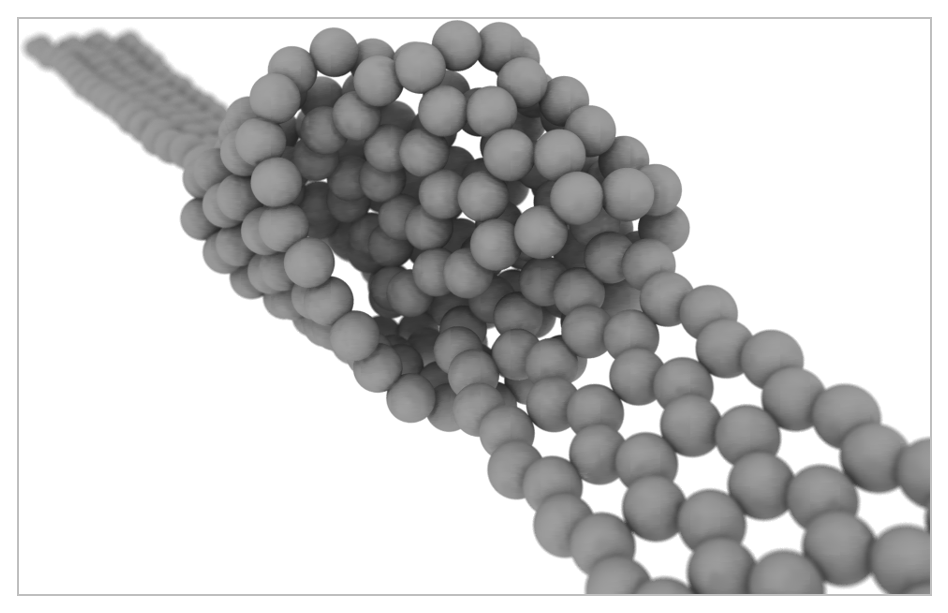
\includegraphics[width=0.48\textwidth]{images/structure}
\end{figure}
\begin{figure}
  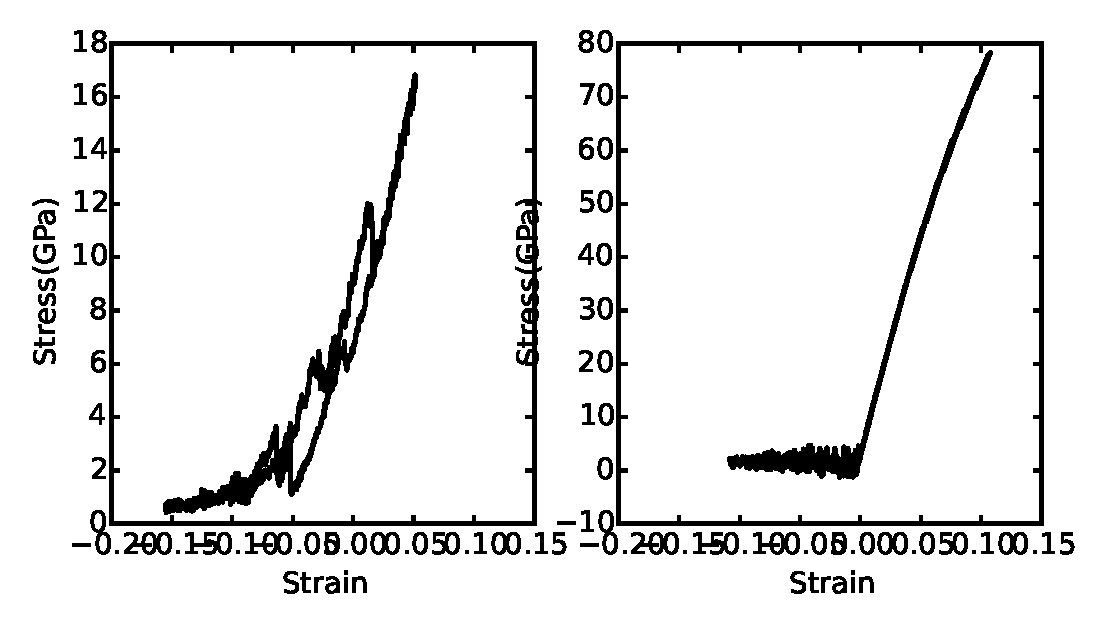
\includegraphics[width=0.48\textwidth]{images/cycle}
\end{figure}
\begin{figure}
  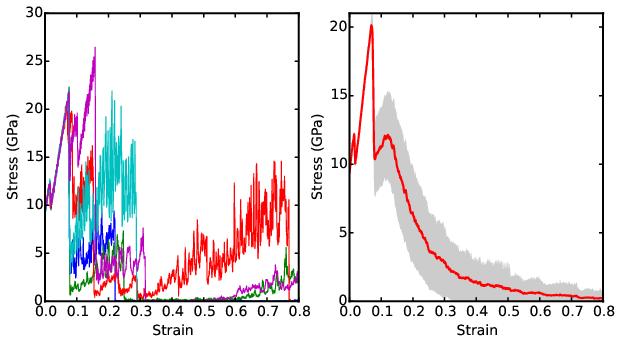
\includegraphics[width=0.48\textwidth]{images/stress}
\end{figure}
\begin{figure}
  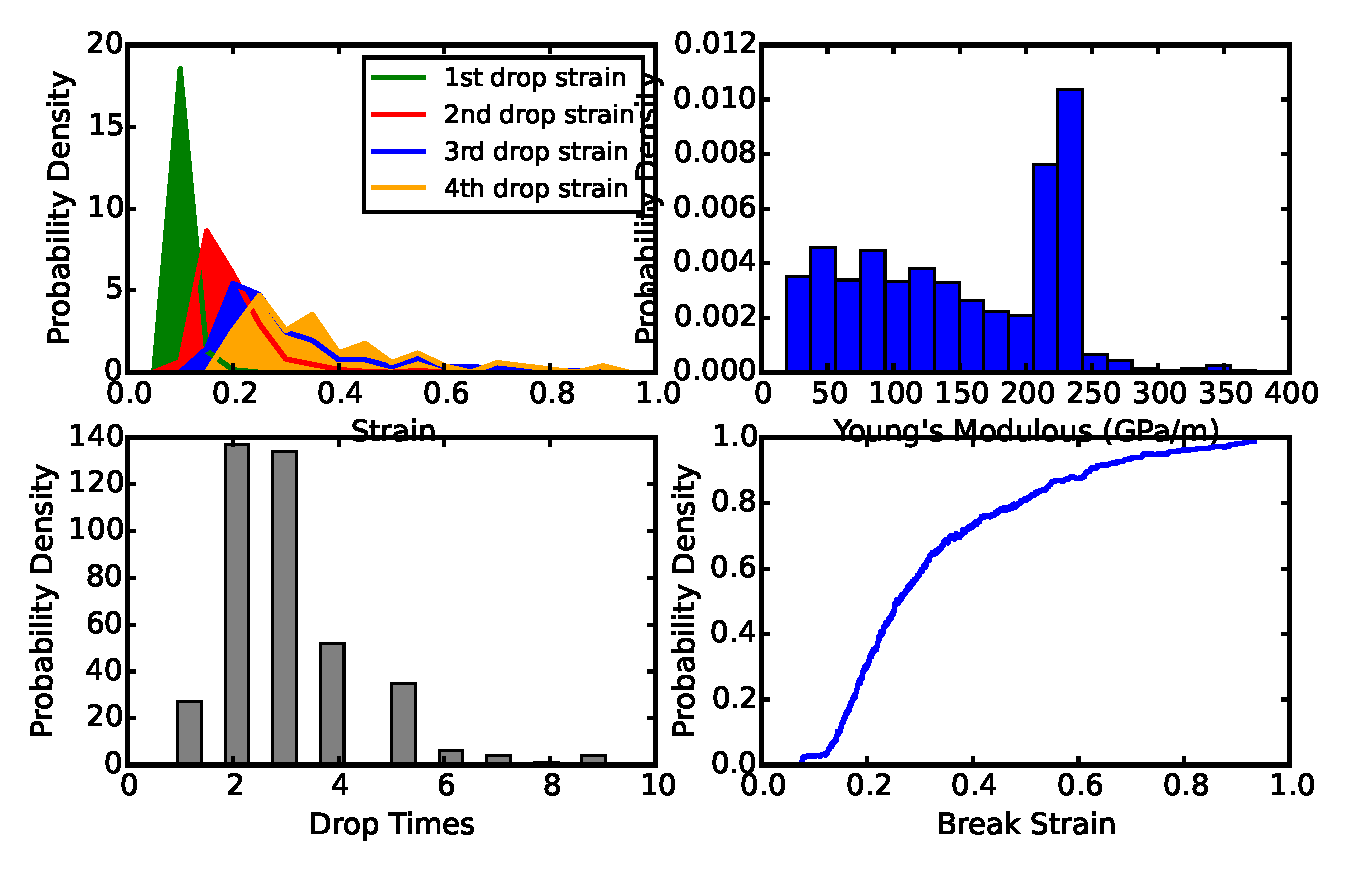
\includegraphics[width=0.48\textwidth]{images/drop}
\end{figure}
\begin{figure}
  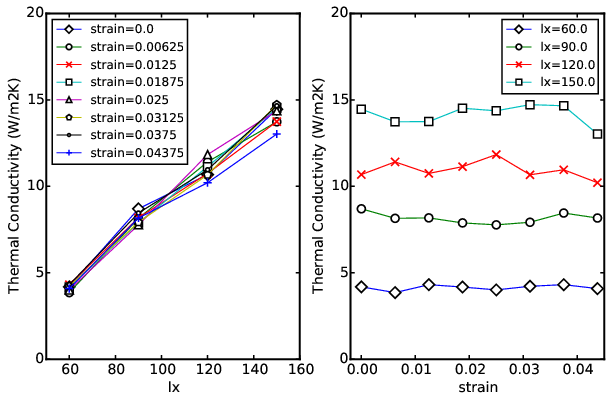
\includegraphics[width=0.48\textwidth]{images/tc_lx}
\end{figure}
\begin{figure}
  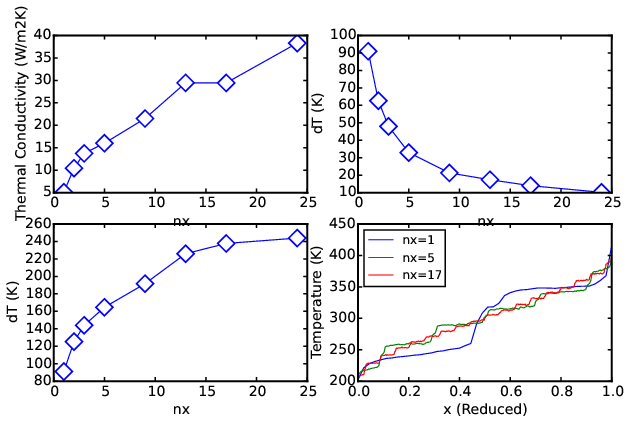
\includegraphics[width=0.48\textwidth]{images/tc_nx}
\end{figure}

\begin{figure}
  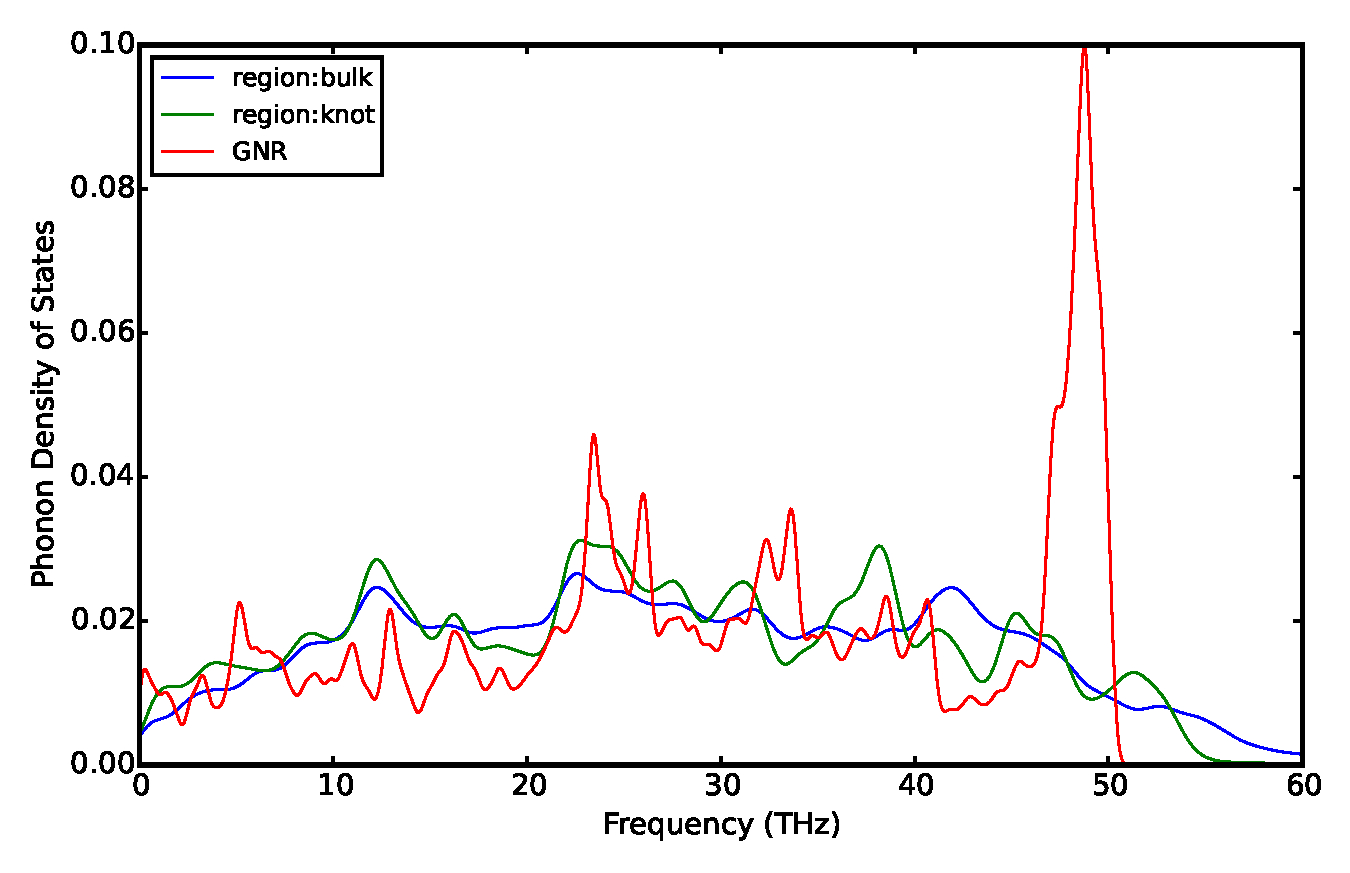
\includegraphics[width=0.48\textwidth]{images/dos}
\end{figure}

\section{CONCLUSIONS}


\quad \\
\section{ACKNOWLEGEMENTS}
This paper was partially supported by the National Natural Science Foundation of China, the Special Funds for Major State Basic Research, the Foundation for the Author of National Excellent Doctoral Dissertation of China, the Program for Professor of Special Appointment at Shanghai Institutions of Higher Learning, and the Research Program of Shanghai Municipality and the Ministry of Education.


\bibliography{ref}
\end{document}